
\documentclass{article}
\usepackage[utf8]{inputenc}
\usepackage{fullpage}
\usepackage{float}
\usepackage{fontspec, xunicode, xltxtra}
\usepackage{amsmath}
\usepackage{amssymb}
\usepackage{mathtools}
\usepackage{color,listings}
\usepackage{mathtools}
\usepackage{graphicx}
\usepackage{grffile}
\usepackage{setspace}              % setspace package: /begin{spacing}{}
\usepackage[margin=1in]{geometry}  % geometry package: left right top height width
\usepackage{color}                 % text decorations require 
\usepackage{soul}                  % text decorations require
\usepackage[export]{adjustbox}
%\setmainfont{Hiragino Sans GB}    % for text including chinese characters
\usepackage{dcolumn}  
\usepackage{array}
\usepackage{subcaption}
\usepackage[justification=centering]{caption}
\usepackage[shortlabels]{enumitem}
\usepackage [english]{babel}
\usepackage [autostyle, english = american]{csquotes}
\MakeOuterQuote{"}
\usepackage{hyperref}
\hypersetup{
    colorlinks=true,
    linkcolor=blue,
    filecolor=magenta,      
    urlcolor=cyan,
}
\usepackage{geometry}
\geometry{
letterpaper,
tmargin=.5cm,
bmargin=.5cm,
lmargin=2cm,
rmargin=2cm
}


\renewcommand{\thesubsection}{\alph{subsection}}
\newenvironment{Step}{%
    \begin{enumerate}[label= \textbf{Step \arabic*},align=left, leftmargin=1.6cm]%
}{
    \end{enumerate}%
}


\newcolumntype{$}{>{\global\let\currentrowstyle\relax}}
\newcolumntype{^}{>{\currentrowstyle}}
\newcommand{\rowstyle}[1]{\gdef\currentrowstyle{#1}%
  #1\ignorespaces
}
 
\definecolor{codegreen}{rgb}{0,0.6,0}
\definecolor{codegray}{rgb}{0.5,0.5,0.5}
\definecolor{codepurple}{rgb}{0.58,0,0.82}
\definecolor{backcolour}{rgb}{0.95,0.95,0.92}
\lstdefinestyle{mystyle}{
    backgroundcolor=\color{backcolour},   
    commentstyle=\color{codegreen},
    keywordstyle=\color{magenta},
    numberstyle=\tiny\color{codegray},
    stringstyle=\color{codepurple},
    basicstyle=\footnotesize,
    breakatwhitespace=false,         
    breaklines=true,                 
    captionpos=b,                    
    keepspaces=true,                 
    numbers=left,                    
    numbersep=5pt,                  
    showspaces=false,                
    showstringspaces=false,
    showtabs=false,                  
    tabsize=2
}
 
\lstset{style=mystyle}


\title{\Large{Executive Summary of Commercial Analysis}\vspace{-0.5cm}}
\author{Bingxi Li}
\date{\vspace{-2ex}May 2016}
\graphicspath{{./}}

\begin{document}

\begin{singlespacing}

\maketitle
\begin{abstract}
The k-nearest neighbor, logistic regression and Support Vector Machine (SVM) algorithm with kernel method are tuned to predict customer behavior. The performance of these models are compared in terms of accuracy and receiver operating characteristic (roc). The SVM using radial basis function kernel gives most reliable prediction. 
\end{abstract}

\section{Introduction}
A robust model should be trained based on the training data from a company to predict if a customer will buy the product in the future or not. The training data set has \textbf{4} features and \textbf{3089} pieces of records. The predictor will be either \textbf{1} or \textbf{0} given a new \textbf{4} dimension feature.

\section{Methodology and Result}
\subsection{preprocessing}
The features are standardized before training. 30\% of the records are hold out as \textbf{test\ set} while the rest records are use as \textbf{train\ set} to tune knn and logistic model and SVM model. The latter two of the three models are tuned with different kernel through 5-fold cross validation. The best model are selected among these tuned ones based on their predictabilities to the same test set. The details about implementation are included in the attached "training.py".

\subsection{K-Nearest Neighbor}
Ranging from 1 to 24 stepped by 1, the number of nearest neighbors, K, at \textbf{1} yields highest accuracy. The KNN model with K = 1.0 is then trained with whole \textbf{train set} to predict \textbf{test set}. The accuracy is \textbf{0.95361}.

\subsection{logistic regression}
Ranging from 0.5 to 50 with step size being 0.5, the inverse of regularization strength, C, at \textbf{7.0} yields highest mean score through 5-fold cross-validation. The Logistic regression model with C = 1.0 is then trained with  whole \textbf{train set} and to predict \textbf{test set}. The following is summary of precision, recall, F1 score for each class.
\begin{lstlisting}
             precision    recall  f1-score   support
        0.0    0.93354   0.92767   0.93060       318
        1.0    0.96236   0.96552   0.96393       609
avg / total    0.95247   0.95254   0.95250       927
\end{lstlisting}
The accuracy given by the best logistic model is \textbf{0.95254}. The quality of this model is also determined with receiver operating characteristic (ROC) curve and precision-recall (PR) curve in Figure ~\ref{fig:logit} (left). The area under curve (AUC) is 0.98941, which indicates very high probability that the classifier will assign a higher score to a randomly chosen positive example than to a randomly chosen negative example.

\subsection{support vector machine}
\subsubsection{with linear kernel}
Ranging from 0.1 to 5.0 with step size being 0.1, penalty parameter C of the error term at \textbf{1.1} and yield highest mean score through 5-fold cross-validation. The linear SVM model with C = 1.1 is then trained with  whole \textbf{train set} and to predict \textbf{test set}. The following is summary of precision, recall, F1 score for each class.
\begin{lstlisting}
             precision    recall  f1-score   support
        0.0    0.94654   0.94654   0.94654       318
        1.0    0.97209   0.97209   0.97209       609
avg / total    0.96332   0.96332   0.96332       927
\end{lstlisting}
The accuracy given by the best linear SVM model is \textbf{0.96332}. The quality of this model is also determined with ROC and PR curve in Figure ~\ref{fig:lsvm}. The AUC is \textbf{0.99034}, which indicates the reliable prediction of this model.


\subsubsection{with radial basis function(rbf) kernel}
Separately ranging from 0.1 to 5.0 stepped by 0.1 and from 0.1 to 1.9 stepped by 0.2, penalty parameter C of the error term at \textbf{4.7} and kenel coefficient $\gamma$ at \textbf{1.1} yield highest mean score through 5-fold cross-validation. The rbf SVM model with C = 4.7 and $\gamma = 1.1 $ is then trained with  whole \textbf{train set} and to predict \textbf{test set}. The following is summary of precision, recall, F1 score for each class.
\begin{lstlisting}
             precision    recall  f1-score   support
        0.0    0.97134   0.95912   0.96519       318
        1.0    0.97879   0.98522   0.98200       609
avg / total    0.97624   0.97627   0.97623       927
\end{lstlisting}
The accuracy given by the best rbf SVM model is \textbf{0.97627}. The quality of this model is also determined with ROC and PR curve in Figure ~\ref{fig:rsvm}. The AUC is \textbf{0.99592} under ROC curve, which indicates the perfect predictability of the model.

\subsubsection{with polynomial kernel}
Separately ranging from 0.1 to 5.0 stepped by 0.1 and from 1 to 4 stepped by 1, penalty parameter C of the error term at \textbf{3.7} and kenel coefficient $\gamma$ at \textbf{3} yield highest mean score through 5-fold cross-validation. The polynomial SVM model with C = 3.7 and $\gamma = 3 $ is then trained with  whole \textbf{train set} and to predict \textbf{test set}. The following is summary of precision, recall, F1 score for each class.
\begin{lstlisting}
             precision    recall  f1-score   support
        0.0    0.98039   0.94340   0.96154       318
        1.0    0.97101   0.99015   0.98049       609
avg / total    0.97423   0.97411   0.97399       927
\end{lstlisting}
The accuracy given by the best polynomial SVM model is \textbf{0.97411}. The quality of this model is also determined with ROC and PR curve in Figure ~\ref{fig:psvm}. The AUC is \textbf{0.99563} under ROC curve, which indicates that SVM with polynomial kernel is also a perfect predict model.

\subsubsection{with sigmoid kernel}
Separately ranging from 0.1 to 5.0 stepped by 0.1 and from 1 to 4 stepped by 1, penalty parameter C of the error term at \textbf{0.2} and kenel coefficient $\gamma$ at \textbf{0.1} yield highest mean score through 5-fold cross-validation. The sigmoid SVM model with C = 0.1 and $\gamma = 0.2 $ is then trained with  whole \textbf{train set} and to predict \textbf{test set}. The following is summary of precision, recall, F1 score for each class.
\begin{lstlisting}
             precision    recall  f1-score   support
        0.0    0.88554   0.92453   0.90462       318
        1.0    0.95966   0.93760   0.94850       609
avg / total    0.93424   0.93312   0.93345       927
\end{lstlisting}
The accuracy given by the best polynomial SVM model is \textbf{0.93312}. The quality of this model is also determined with ROC and PR curve in Figure ~\ref{fig:ssvm}. The AUC is \textbf{0.98352} under ROC curve, which indicates that SVM with polynomial kernel is also a perfect predict model.

\section{Conclusion}
Through this study, the SVM with polynomial kernel and radial basis function(rbf) kernel have similarly perfect prediction. SVM with linear kernel is also good. The KNN and logistic seems less favorable here while sigmoid SVM is probably not a good choice for this prediction.\\

\noindent The SVM using rbf kernel is implemented in \textbf{testing.py} with the optimal parameters given above, C = 4.7 and $\gamma = 1.1$. For future prediction of any new 4-feature data, this model is trained with the data from exam.dat.txt. The attached "testing.py" implemented the above idea using a vector like "F1 F2 F3 F4" or a test file like "test.dat.txt" as input. When used a test file as the input, the file should be in the same format of "exam.dat.txt". Output will be an either 1 or 0 predictor or an array of either 1 or 0 predictors.

\begin{lstlisting}
# use a four feature vector as input
python testing.py F1 F2 F3 F4
#[1.]

# use a test data file as input
python testing.py "test.dat.txt"
#[1. 1. 0. ....]
\end{lstlisting}

\newpage
\section{Reference}

\begin{figure}[H]
    \centering
    \begin{subfigure}[b]{0.4\textwidth}
        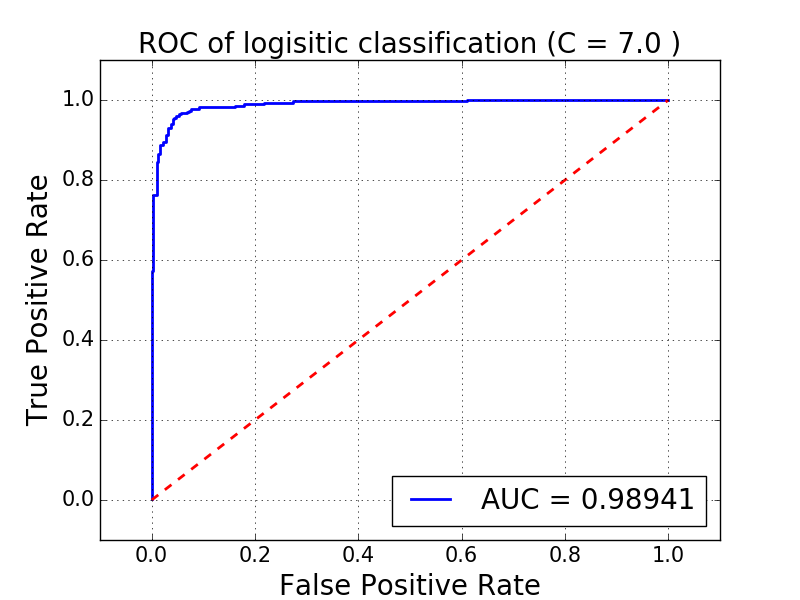
\includegraphics[width=\textwidth]{logistic_roc.png}
    \end{subfigure}
    \begin{subfigure}[b]{0.4\textwidth}
        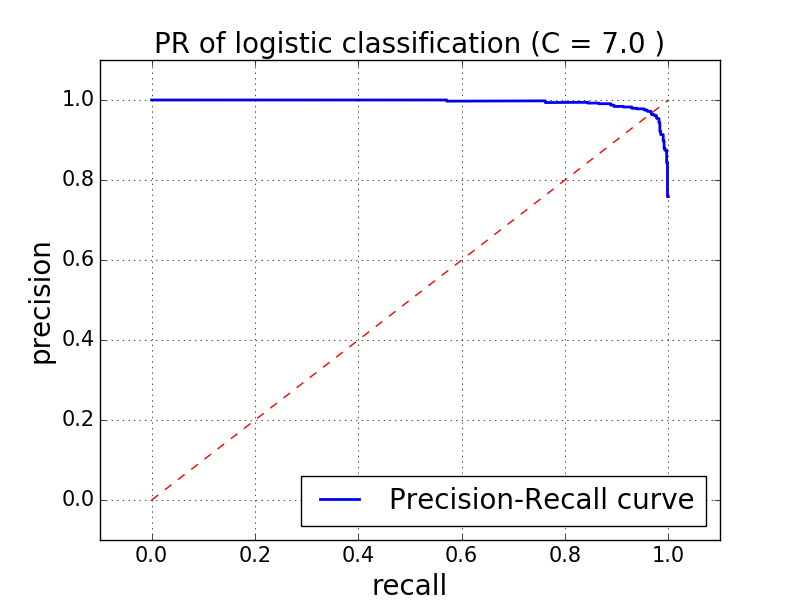
\includegraphics[width=\textwidth]{logistic_pr.png}
    \end{subfigure}
    \caption{ROC curve(left) and PR curve(right) by logistic prediction}\label{fig:logit}
\end{figure}

\begin{figure}[H]
    \centering
    \begin{subfigure}[b]{0.4\textwidth}
        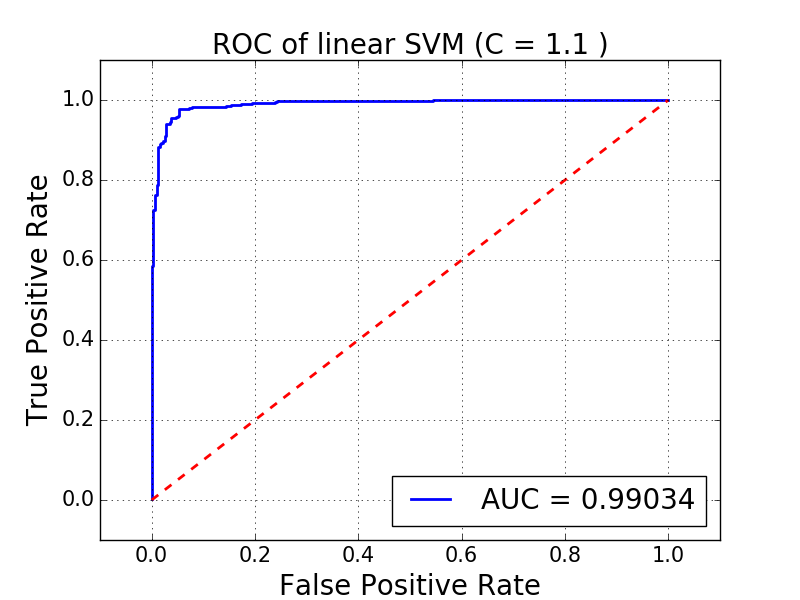
\includegraphics[width=\textwidth]{lsvm_roc.png}
    \end{subfigure}
    \begin{subfigure}[b]{0.4\textwidth}
        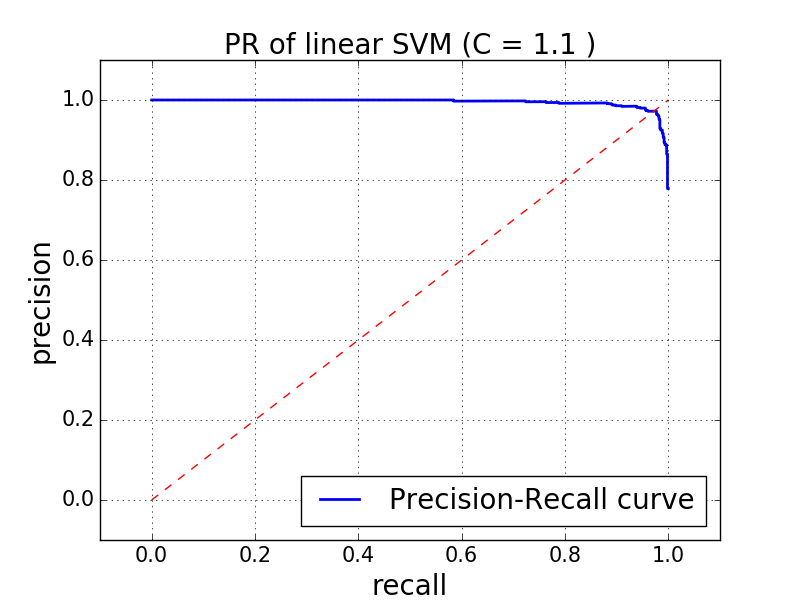
\includegraphics[width=\textwidth]{lsvm_pr.png}
    \end{subfigure}
    \caption{ROC (left) and PR curve(right) by linear SVM prediction}\label{fig:lsvm}
\end{figure}

\begin{figure}[H]
    \centering
    \begin{subfigure}[b]{0.4\textwidth}
        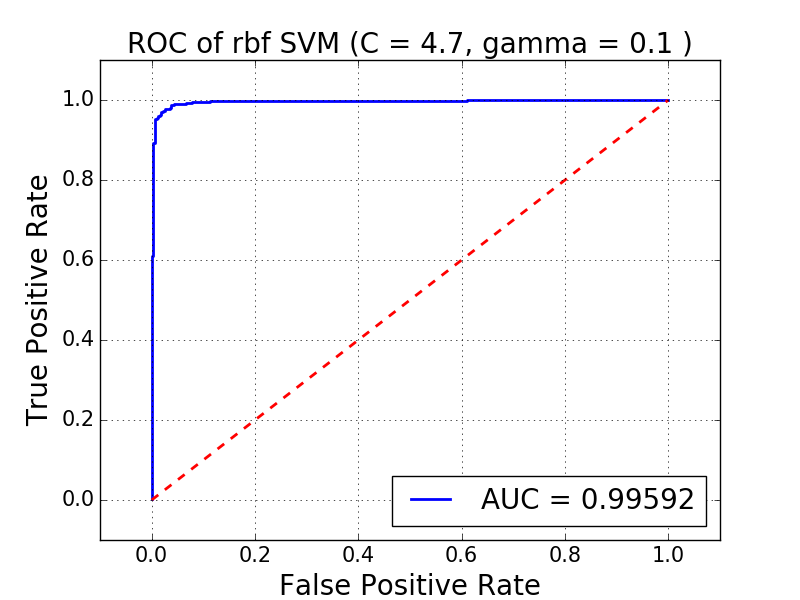
\includegraphics[width=\textwidth]{rsvm_roc.png}
    \end{subfigure}
    \begin{subfigure}[b]{0.4\textwidth}
        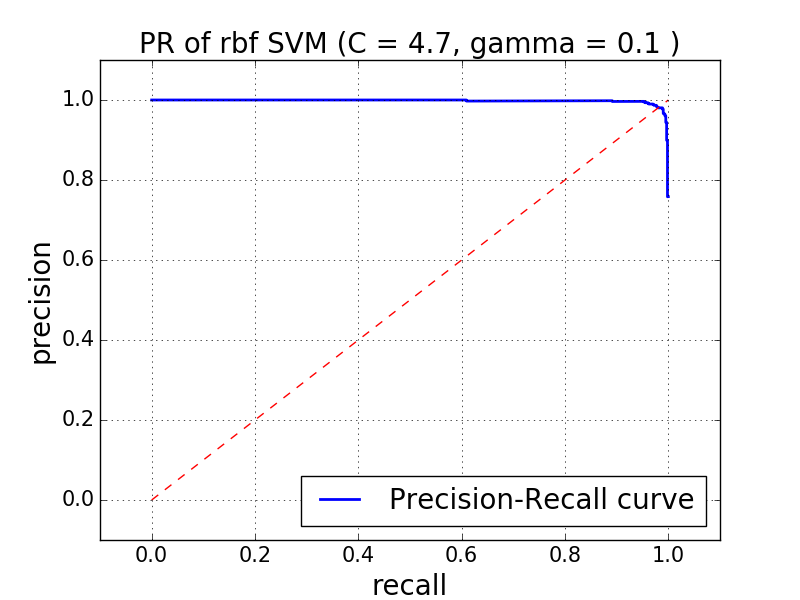
\includegraphics[width=\textwidth]{rsvm_pr.png}
    \end{subfigure}
    \caption{ROC (left) and PR curve(right) by rbf SVM prediction}\label{fig:rsvm}
\end{figure}

\begin{figure}[H]
    \centering
    \begin{subfigure}[b]{0.4\textwidth}
        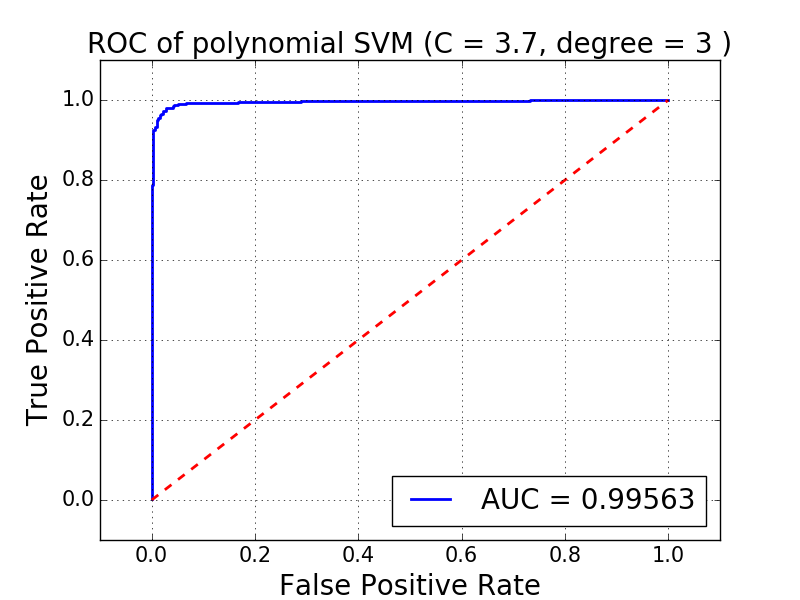
\includegraphics[width=\textwidth]{psvm_roc.png}
    \end{subfigure}
    \begin{subfigure}[b]{0.4\textwidth}
        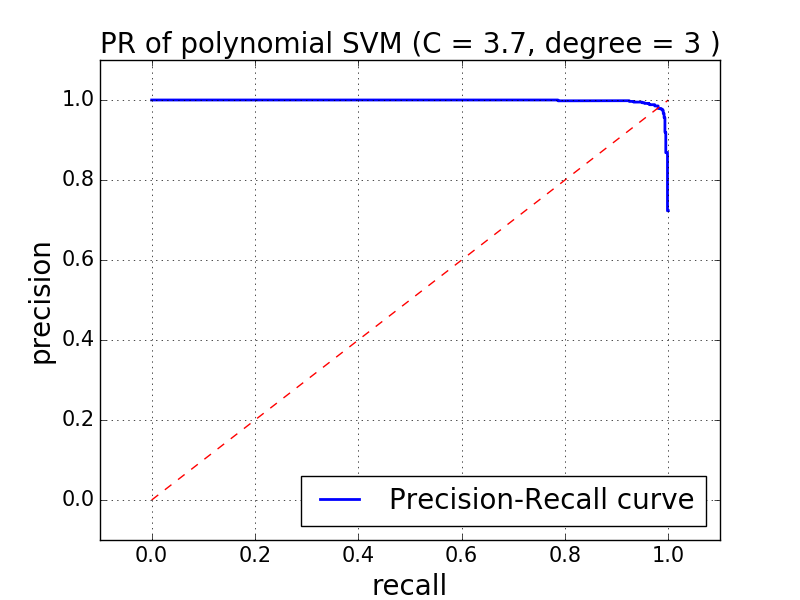
\includegraphics[width=\textwidth]{psvm_pr.png}
    \end{subfigure}
    \caption{ROC (left) and PR curve(right) by polynomial SVM prediction}\label{fig:psvm}
\end{figure}

\begin{figure}[H]
    \centering
    \begin{subfigure}[b]{0.4\textwidth}
        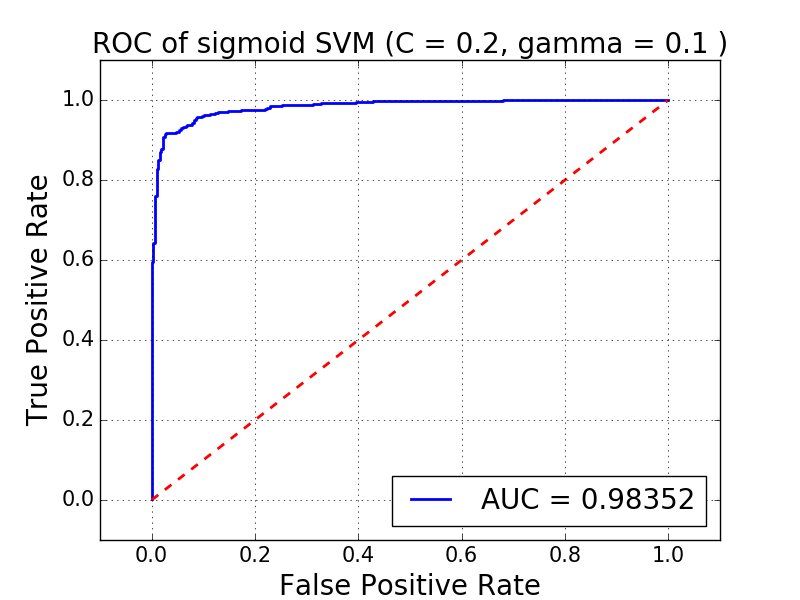
\includegraphics[width=\textwidth]{ssvm_roc.png}
    \end{subfigure}
    \begin{subfigure}[b]{0.4\textwidth}
        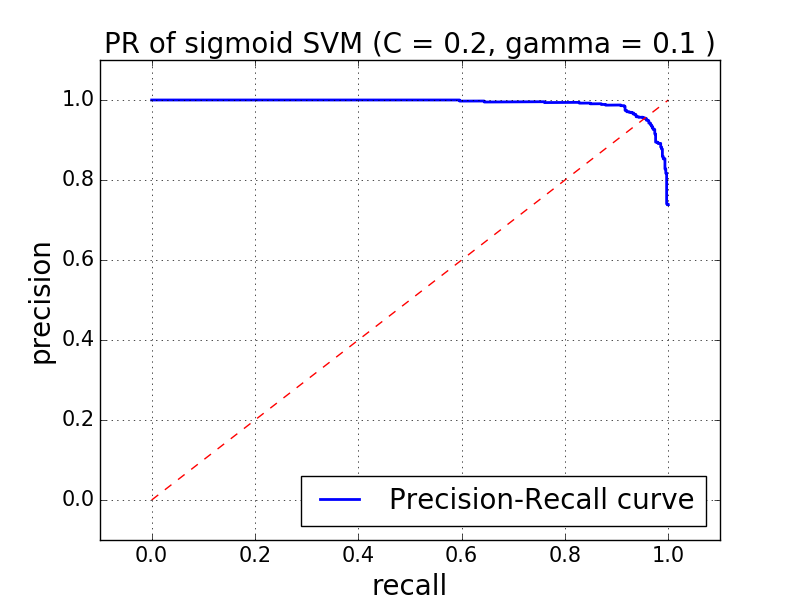
\includegraphics[width=\textwidth]{ssvm_pr.png}
    \end{subfigure}
    \caption{ROC (left) and PR curve(right) by sigmoid SVM prediction}\label{fig:ssvm}
\end{figure}



\end{singlespacing}
\end{document}